\documentclass[conference]{IEEEtran}
\usepackage[T1]{fontenc} %%%key to get copy and paste for the code!
\usepackage[utf8]{inputenc} %%% to support copy and paste with accents for french stuff
\usepackage{times}
\usepackage[scaled=0.85]{helvet}
\usepackage{graphicx}
\usepackage{ifthen}
\usepackage{xspace}
\usepackage{alltt}
\usepackage{latexsym}
\usepackage{url}
\usepackage{amsmath,amssymb,amsfonts}
\usepackage{stmaryrd}
\usepackage{algorithmic}
\usepackage{textcomp}
\usepackage{xcolor}
\usepackage{enumerate}
\usepackage{cite}
\usepackage[pdftex,colorlinks=true,pdfstartview=FitV,linkcolor=blue,citecolor=blue,urlcolor=blue]{hyperref}
\usepackage{multirow}


% natbib
\usepackage[numbers]{natbib}
\newboolean{showcomments}
\setboolean{showcomments}{true}
\ifthenelse{\boolean{showcomments}}
  {\newcommand{\bnote}[2]{
	\fbox{\bfseries\sffamily\scriptsize#1}
    {\sf\small$\blacktriangleright$\textit{#2}$\blacktriangleleft$}
    % \marginpar{\fbox{\bfseries\sffamily#1}}
   }
   \newcommand{\cvsversion}{\emph{\scriptsize$-$Id: macros.tex,v 1.1.1.1 2007/02/28 13:43:36 bergel Exp $-$}}
  }
  {\newcommand{\bnote}[2]{}
   \newcommand{\cvsversion}{}
  } 


\newcommand{\here}{\bnote{***}{CONTINUE HERE}}
\newcommand{\nb}[1]{\bnote{NB}{#1}}

\newcommand{\fix}[1]{\bnote{FIX}{#1}}
%%%% add your own macros 

\newcommand{\ab}[1]{\bnote{Alex}{#1}}
\newcommand{\sd}[1]{\bnote{Stef}{#1}}
\newcommand{\ja}[1]{\bnote{Jannik}{#1}}
\newcommand{\md}[1]{\bnote{MD}{#1}}
\newcommand{\jr}[1]{\bnote{JRe}{#1}}
\newcommand{\lf}[1]{\bnote{Luc}{#1}}
\newcommand{\na}[1]{\bnote{Nic}{#1}}
\newcommand{\an}[1]{\bnote{Anne}{#1}}
\newcommand{\bv}[1]{\bnote{Benoit}{#1}}

\graphicspath{{figures/}}
%%% 


\newcommand{\figref}[1]{Figure~\ref{fig:#1}}
\newcommand{\figlabel}[1]{\label{fig:#1}}
\newcommand{\tabref}[1]{Table~\ref{tab:#1}}
\newcommand{\layout}[1]{#1}
\newcommand{\commented}[1]{}
\newcommand{\secref}[1]{Section \ref{sec:#1}}
\newcommand{\seclabel}[1]{\label{sec:#1}}

%\newcommand{\ct}[1]{\textsf{#1}}
\newcommand{\stCode}[1]{\textsf{#1}}
\newcommand{\stMethod}[1]{\textsf{#1}}
\newcommand{\sep}{\texttt{>>}\xspace}
\newcommand{\stAssoc}{\texttt{->}\xspace}

\newcommand{\stBar}{$\mid$}
\newcommand{\stSelector}{$\gg$}
\newcommand{\ret}{\^{}}
\newcommand{\msup}{$>$}
%\newcommand{\ret}{$\uparrow$\xspace}

\newcommand{\myparagraph}[1]{\noindent\textbf{#1.}}
\newcommand{\eg}{\emph{e.g.,}\xspace}
\newcommand{\ie}{\emph{i.e.,}\xspace}
\newcommand{\etal}{\emph{et al.,}\xspace}
\newcommand{\ct}[1]{{\textsf{#1}}\xspace}


\newenvironment{code}
    {\begin{alltt}\sffamily}
    {\end{alltt}\normalsize}

\newcommand{\defaultScale}{0.55}
\newcommand{\pic}[3]{
   \begin{figure}[h]
   \begin{center}
   \includegraphics[scale=\defaultScale]{#1}
   \caption{#2}
   \label{#3}
   \end{center}
   \end{figure}
}

\newcommand{\twocolumnpic}[3]{
   \begin{figure*}[!ht]
   \begin{center}
   \includegraphics[scale=\defaultScale]{#1}
   \caption{#2}
   \label{#3}
   \end{center}
   \end{figure*}}

\newcommand{\infe}{$<$}
\newcommand{\supe}{$\rightarrow$\xspace}
\newcommand{\di}{$\gg$\xspace}
\newcommand{\adhoc}{\textit{ad-hoc}\xspace}

\usepackage{url}            
\makeatletter
\def\url@leostyle{%
  \@ifundefined{selectfont}{\def\UrlFont{\sf}}{\def\UrlFont{\small\sffamily}}}
\makeatother
% Now actually use the newly defined style.
\urlstyle{leo}






\author{
    \IEEEauthorblockN{Beno\^{i}t Verhaeghe$^{1,2}$, Anne Etien$^1$,\\ Nicolas Anquetil$^1$, St\'{e}phane Ducasse$^1$}\IEEEauthorblockA{$^1$Universit\'{e} de Lille, CNRS, Inria, \\ Centrale Lille, UMR 9189 -- CRIStAL, France\\}
    \and
    \IEEEauthorblockN{Abderrahmane Seriai$^2$, Laurent Deruelle$^2$,\\ Mustapha Derras$^2$}\IEEEauthorblockA{$^2$Berger-Levrault, France}     
}

\begin{document}
\title{GUI application meta-models:\\ a state of the art}


\date{\today}
\maketitle

\begin{abstract}

\bvc{In this context...}
When a developer wants to analyse an application,
    and this application includes an user interface.
He could want an abstraction of the application.
Often, this abstraction level correspond to models, and their meta-models, of
    the piece of software.
\bvc{We consider this problem P...}
There are indeed many elements to represent and to link.
\bvc{P is a problem because...}
Currently there are many meta-models of GUI application
    that can be used to represent the interface
    and some links between the different windows.
But none of them express complex behavior, such as loop or condition,
    nor data structure information.
\bvc{We propose this solution...} 
We defined four meta-models.
The first one represent the Graphical User Interface,
    the second one the layout to apply to the GUI, 
    the third one the data structure implies in the GUI, 
    the last one the behavior associate to an event fired by an element of the GUI. 
\bvc{Our solution solves P in such and such way.}
Our meta-models can express the different elements of a GUI application.
So can represent the graphical user interface
    and the logic of the application.

   
\end{abstract}

\begin{IEEEkeywords}
    Graphical User Interfaces, Model-Driven Engineering
\end{IEEEkeywords}

\section{Introduction}
\label{sec:intro}

% Contexte
\bvc{Contexte} \bvc{use case}
In the context of the analysis of an application.
It happens that the developers want to create tools on top of his analysis.
These tools could be useful in cases like:
    analysis, tests generation, migration, \etc.

\bvc{introduction model}
A way to create those software is the usage of model of the source code of the application.
The developers create or use a meta-model of the language of the application source code.
Then they instantiate this meta-model from the application to analysed.

% Problème
\bvc{Problème}
\bvc{intro gui}
In the case of GUI application, it happens that the abstraction level does not provide enough information.
Indeed, the generated model contains the methods, classes, \etc. of the source application,
    but no information about how the GUI is shaped.
The developers must do another analysis on the model to extract these information and so
    making his tool.

\bvc{intro simple gui decomposition}
A solution to create tool specialized for GUI application is to create GUI model.
A GUI application is divided into different elements.
The aim of this paper is to define those components and meta-models
    to represent all the specificities linked to a GUI application.

% Known tracks for \sd{solutions} here you want to show that you are not an idiot not knowing what have been around
\bvc{Know tracks}
We did not find any other papers which defines a solution to represent graphical application.
Nevertheless, the KDM model designed by the OMG proposed a \textit{Resource Layer} which can used to define an GUI application.
Their solution is discussed section X.

% What our solution is \ct{Set} and \ct{OrderedCollection} (so that the reader knows where the paper is going)
\bvc{What is our solution}
We defined four meta-models to represent the GUI software.
The meta-models represent the different main GUI's specificities we extracted from our analysis
    and other research papers.

% Contribution of the paper
\bvc{Contrib of the paper}
The main contributions of our work are: 

\begin{itemize}
    
    \item Description of GUI application structure

    \item Meta-Models to represent a GUI application

    \item Discussion about GUI Meta-Models

\end{itemize}

% Paper structure
\bvc{Paper structure}
In Section~\ref{sec:guiAppDiv}, we present the different GUI elements
Section~\ref{sec:contribution} exposes our solution.
Then, In Section~\ref{sec:solutions}, we describe and categorized the solution proposed 
    by others authors.
Finally, we conclude in Section~~\ref{sec:conclusion}.

\section{GUI application structure}
\label{sec:guiAppDiv}

The first step to create the meta-models of a graphic application
    is to define the elements we need to represent.
We divided the UI into the following three parts:

\begin{itemize}
    \item The user interface
    \item The business code
    \item The behavior code 
\end{itemize}

\subsection{User Interface}
\label{sec:userInterface}

The user interface is the viewable part.
This element represents the interface of the application.
It includes the components of the interface.
The User Interface does not contain the exact visualisation of a component.
But it can precise some feature inherent to the component, like the ability to be clicked,
    or some properties of the component, like its color or size.
More than the components, it also includes the disposition
    of those components in relation to the others.
In the case a application is composed by multiple windows (or web pages for web application),
    the user interface contains all the windows.

\subsection{Behavior Code}
\label{sec:behaviorCode}

The behavior code is the \textit{executable} part of the application.
It corresponds to the logic of the application.
It can have two manifestations of the business code.
It can be run either by an user action on an interface component (like a click)
    or by the system itself.
As a programming language, the business code contains control structures
    (\ie loop and alternative).
Linked to the user interface, the business code defined the logic of the user interface.
However, the business code does not express the logic of the application.
This part is dedicated to the business code. 

\subsection{Business Code}
\label{sec:businessCode}

The business code defines specific information of an application.
It is composed by the general rules of the application
    (how calculate the taxes?),
    the distant services link (which server my business code should request),
    the data of the application (which database? which kind of \textit{object}?).
So the business code is not directly linked to the user interface. 

\section{Proposed meta-models}
\label{sec:contribution}

From the decomposition of the GUI application structure (see Section~\ref{sec:guiAppDiv}),
    we decided to create four meta-models.

\begin{itemize}
    \item The GUI model
    \item The layout model
    \item The business model
    \item The behavior model
\end{itemize}


\subsection{The GUI model}
\label{sec:guiModel}

In order to represent a GUI, we designed a meta-model presented \figref{guiModel}.
This GUI model is the first part of the user interface component of
    a graphic application as defined Section~\ref{sec:userInterface}
In the following, we present the different entities of the meta-model.

\pic{figures/GUIModel.png}{GUI Application Metamodel}{fig:guiModel}


The \textbf{Phase} represents the main container of a user interface page.
It can be a \textit{Window} for Desktop application,
    a web page or a tab in some specific case.
For example, 
    if a web site is composed by only one web page, 
    and this web page has multiple tab.
To represent the website as the content of the different tabs, 
    the Phases will represent a tab.
A Phase can contains multiple Business Page.
It can also be called by any Widget with a \textit{Call Phase Action}.
When a Phase is called, the interface changes to display the phase.
In desktop application, the current Window interface changes from the previous Phase to 
    the called one or a new Window with the interface owned by the called Phase is opened.
In web application, it can be a new web page, the changement of active tab, the transformation of the current web page. 

The \textbf{Widgets} are the different interface components and layout components.
There are two types of Widgets.
The \textbf{Leaf} is a widget which does not contain another widget such as some text in the interface. 
The \textbf{Containers} can contain other widget. 
It could be for organization purposed like separating widgets which belongs to a category and widgets which belongs to another category.

The \textbf{Business Pages} blabla \bv{Très BL specific... Il faudrait supprimer Page Métier}.

The \textbf{Attribute} represents informations that belongs to a Widget and can change its visual aspect or its behavior.
The common attributes are the height and the width to define precisely the dimension of a widget.
There are also attributes to contains attributes such as the text contained by a widget. 
For example, a widget which represent a button can have an attribute \textit{text} to 
    explicit the text of the button.
An attribute can change the behavior, it could be the case of an attribute \textit{enable}.
A button with the attribute \textit{enable} positioned at \textit{false} represent a button
    we can not click.

The \textbf{Actions} are own by the Widgets.
They are actions that can be run in a Graphic Interface.

\bv{Should disapear and be splitted between Business and behavior model}
\textbf{Call Service} represents a call to a distant service such Internet.
\textbf{Fire PopUp} is the action that display a PopUp in the screen.
The PopUp can not be considered as a Widget, 
    it is not present in the GUI, 
    it only appears and disappears.

\bv{SHOUDL Disapear and go to the Behavior Model}The \textbf{Service} is the reference to the distant feature the application can call from its GUI.
In a web context, it can be the server side of the application.

\subsection{The layout model}
\label{sec:layoutModel}

\bv{Ajouter un layout model}

The layout model is the second part of the user interface defined Section~\ref{sec:userInterface}.
It contains the information concerning the visual disposition of the elements of the user interface.
It does not include properties as color or text size of an element.
The aim of the layout model is to explicit the layout applied by a \textit{container widget}.
It exists some common layout as \textbf{HorizontalLayout}, \textbf{VerticalLayout} or \textbf{GridLayout}.
Each widget can only have one layout,
    but because a \textit{container} can contain another \textit{container},
    it is possible to define complex layout composition.



\subsection{The behavior model}
\label{sec:behaviorModel}
    
% \pic{figures/BehaviorModel.png}{Behavior Metamodel}{fig:behaviorModel}

\begin{figure}
    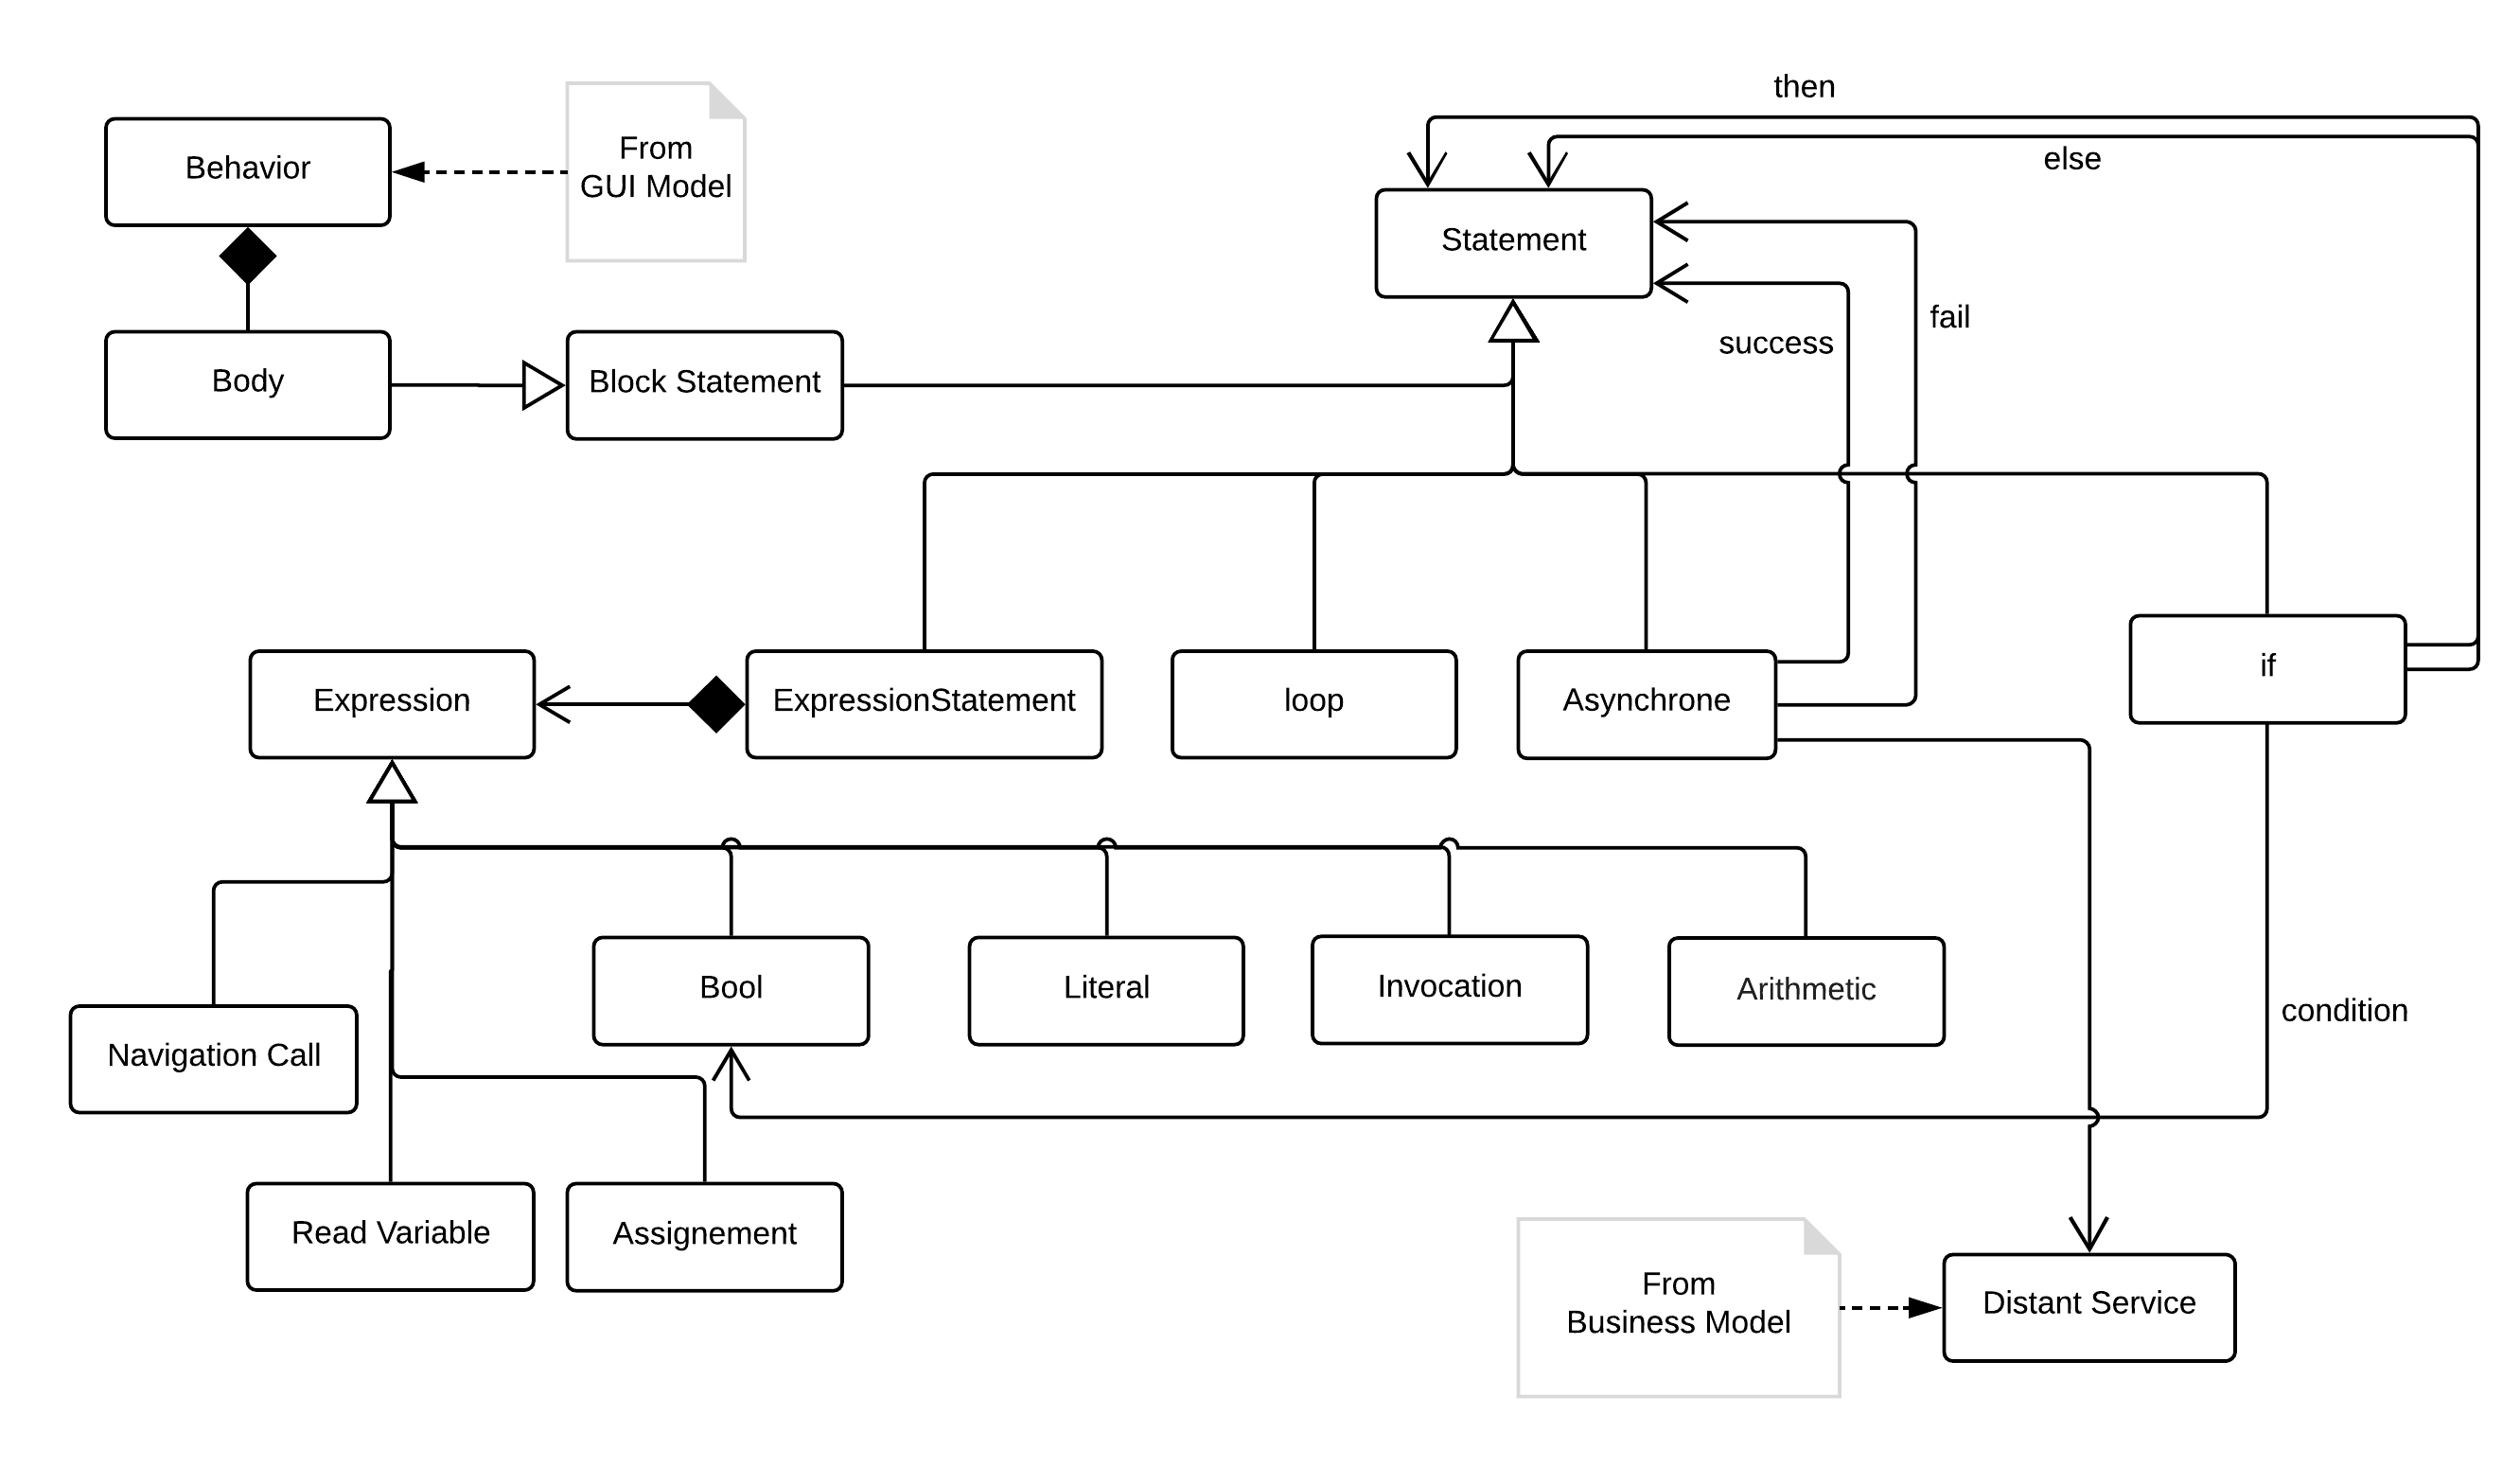
\includegraphics[width=\linewidth]{figures/BehaviorModel.png}
    \caption{Behavior Metamodel}
    \label{fig:behaviorModel}
\end{figure}

The behavior model presented \figref{behaviorModel} is the owner of
    the behavior code.
There are two main elements, ths statement and the expression.

The \textbf{Statement} is the representation of the control structures of
    a programming language.
There are the alternative, the loop, the notion of block and a link to an expression.

The \textbf{Expression} represents a piece of code that can be valued directly.
So it can be an assignment with the value of the assignment,
    a literal (\ie directly the value of the written element),
    a boolean expression, 
    an arithmetic expression
    or an invocation.
In the case of an invocation, it is the return value of the called method that
    is used as the value of the expression.

The \textbf{Behavior} elements is the link to the GUI model.
It is the container of the logic of an event fired by an action.

Thanks to this model, we are able to represent the logic to execute once an user
    fire an event from an action on a widget of the GUI model.



\subsection{The business model}
\label{sec:businessModel}  

\bv{Ajouter un business model}
The business model contains two main composites of the application.
The data and the information about the distant services.

\subsection{Model View Controller}
\label{sec:mvc}

We made a comparaison between our proposed models and the MVC pattern.
The \tabref{mvcMatching} present the matching between the models.

\begin{table}[hbtp]
    \caption{Linked between ours model and the MVC pattern}
    \label{tab:mvcMatching}
    \begin {center}
%    \resizebox{\columnwidth}{!}{%
    \begin{tabular}{|l|l|}
        \hline
         MVC & Ours Models \\
        \hline
        Model & Business \\
        \hline
        \multirow{2}*{View} & Layout \\
        \cline{2-2}
         & GUI \\
        \hline
        Controler & Behavior \\
        \hline
    \end{tabular} %
 %   }
    \end{center}
    \end{table}

\section{Existing solutions}
\label{sec:solutions}

% Context, exposed with the \textbf{most precise terms possible} (don't open
% unwanted doors for the reader)

\bvc{intro expliquand ce que l'on va faire (analyse des modèles)}
Many authors have tried to represent a GUI application.
They created meta-models that define the entities
    they need for their analysis.
Those models helped us to define meta-models to represent any GUI applications.
We analysed and grouped the meta-models of 14 relevant papers in the
    GUI application representation field.
 
\subsection{GUI}
\label{sec:gui}

\begin{table}[hbtp]
\caption{GUI elements}
\label{tab:guiElements}
\begin{center}
%\resizebox{\columnwidth}{!}{%
    \begin{tabular}{|c|c|}
        \hline
        SubWidgets & \citep{gotti2016java,sanchez2014model, memon2007eventflow} \\
        \hline
        Events & \citep{gotti2016java, fleurey2007model, morgado2011reverse, garces2017white, memon2007eventflow, samir2007swing2script, joorabchi2012reverse,  amalfitano2012using, silva2010guisurfer} \\
        \hline
        Properties & \citep{gotti2016java, sanchez2014model, morgado2011reverse, garces2017white, memon2007eventflow, samir2007swing2script, shah2011reverse, joorabchi2012reverse, MemonWCRE2003, mesbah2012crawling, amalfitano2012using, silva2010guisurfer} \\
        \hline
    \end{tabular} %
%}
\end{center}
\end{table}

\bvc{presenter en quelques lignes tout les modèles proposés}
\citet{gotti2016java} proposed a meta-model inspired by KDM model (see Section~\ref{sec:kdm}).
The model has the main entities we also defined.
There is the composite pattern to represent the DOM of a graphic interface.
Their widget are called \textit{Component} and as us they have properties.
They also implemented an event property for the widget. 
But they inverse the name \textit{event} and \textit{action} compare to our solution.

\citet{fleurey2007model} did not show the GUI meta-model directly but
    we extracted information from their navigation model (see \ref{sec:navigation}).
They have, at least, two elements in their GUI model that represent a \textit{Window}
    and a \textit{GraphicElement}.
The Window seems to correspond to our phase entity.
And because the \textit{GraphicElement} and the \textit{Window} are not linked,
    we can supposed that the \textit{GraphicElement} is a widget.
The \textit{GraphicElement} has an \textit{Event}.
We do not have the totality of the GUI meta-model,
    but we can see that it is next to our.

The GUI meta-model of \citet{sanchez2014model} is simple 
    and very similar to our.
It has the entities Widget and Window which correspond respectively to
    our Widget and Phase.
Their Widget has their x and y position and their width and height as properties.
It is similar to the link between Widget and Attribute in our meta-model.
There is also the composite pattern to represent the DOM.

\citet{morgado2011reverse} used a GUI meta-model but do not describe it.
We only know that the GUI is represented as a tree which is similar to
    the DOM and can be represented thank to the composite pattern.

The GUI meta-model of \citet{garces2017white} differs a lot from our.
There are the attributes, the events, the screen (which is like a Phase)
    but there is not widget.
This absent is explained by the difference of source technology.
The authors worked on a project that used oracle forms.
This technology is used to create simple interface with only
    textfield or form.
The textfield contains data from a database.
The disposition of the elements is also really simple in the example provides
    by the authors because the textfield or form are displayed each below each other.
We still can notice that they use an event entity to represent the action of the user with the
    user interface.

\citet{MemonWCRE2003} represents a GUI user interface with only two entities in their GUI meta-model.
A GUI window, which is similar to our Phase, is constituted by a set of widget.
Those widgets can have properties and all the properties have a value associate.
They do not have a representation of the DOM because it was not in the scope of
    their work.
The authors defined a user interface as the set of widget and their properties,
    so, if a widget can two different values during the execution of the program, 
    it belongs to two different user interfaces.
This point is the major difference with the meta-models we proposed because,
    in our design if the value of a property change, we still be in the same user interface
    but a behavioral code has been executed.

\citet{samir2007swing2script} worked on the migration of Java-Swing application to Ajax Web application.
They created a meta-model to represent the UI of the original application.
This meta-model is stored in a XUL file and represents
    the widgets with their properties and the layout.
Those widgets belongs to a Window, which is called Phase in our work, and
    can fire event when a GUI input is executed.
In our work, we have the same system for the event but the Input is hidden under the concept of Action.

\citet{shah2011reverse} used a a tree architecture to represent the GUI.
The root of the tree is a \textit{Frame}.
It corresponds to our Phase.
The root contains components with their properties.
The component entity is similar to our Widget entity.

\citet{joorabchi2012reverse} represent an user interface with a set of UI element.
Those elements are our definition of a widget without the container pattern.
For each UI element, the authors' tool are able to handle the detection
    of multiple attributes and of the event linked to the element.

\citet{memon2007eventflow} used a GUI Model to represent the state of an application (see \ref{sec:state}).
As us, they have a widget with properties.
The author made the difference between \textit{widget} and \textit{container},
    it is similar to the use of the container pattern we use.
With the notion of \textit{container}, the author is able to represent a DOM.

\citet{mesbah2012crawling} did not present directly the user interface meta-model they used.
However, they explain that they use a DOM-tree representation to
    analyse different web page.
They also use the notion of event that can be fired.
They use different instances of their UI meta-model to represent the different web page of the application.
Those instances can be compared to our Phase entities.

\citet{amalfitano2012using} designed an Android Application GUI which is similar to ours meta-model.
They have a notion of interface which is similar to our phase.
An interface contains widgets.
The widgets have properties and event right like in our model.
Their event are parameterizable, this notion is in our behavior model.
They do not use a container pattern to represent the DOM.

Finally, \citet{silva2010guisurfer} used a GUI meta-model but did not present it
    in them paper.
However, they explain that they use a GUI AST to detect the fragment that represents the user interface.
We can linked this GUI AST to the container pattern we used in our GUI model.

\subsection{Navigation}
\label{sec:navigation}

\citet{fleurey2007model} created a navigation meta-model to represent the
    transition between the different user interfaces or the forms to complete by the user.
The model is also linked to an entity called \textit{Operation} but not well described.
It still seems to be a way to call specific code to execute.
The navigation meta-model proposed by the authors is similar to our behavior model.

\citet{morgado2011reverse} designed two meta-models for the navigation.
The first one is the windows model.
It contains all the window available in the application.
For each window, it describes the other window that can be reach from the original one.
This describes the navigation between the window in an application.
The second one is the navigation model.
More than the link between the windows,
    this meta-model stores the user action to performed in order to execute the navigation.
All this information are include in our behavior meta-model.

\subsection{State flow}
\label{sec:state}

\subsection{Layout}
\label{sec:layout}

\citet{gotti2016java} used a layout meta-model to represent
    the position of the element in the user interface.
The authors have chosen the meta-model designed by KDM.
We described the meta-model \secref{kdm}.

\citet{sanchez2014model} designed three layouts meta-models.
The authors made this hight level of decomposition because their case study.
The case study was the reverse engineering of a graphic application developed
    with Rapid Application Development (RAD).
The RAD often implies the non-usage of \textit{common layout}.
So, the authors had to find a way to extract the position of the ui element
    without using \textit{HorizontalLayout}, \textit{VerticalLayout}, \etc, but
    finally representing the application with those layout.
\bv{To recheck}
The first model they designed is the Region model.
The Region model defines squares in the user interface that match the widgets of the interface
    and precises the sub-region.
This model is a way to recreate the composite pattern of our GUI model.
The second model is the Tile model.
This model positioned the different regions with others.
If a region is inside another, it precises the position of the sub-region (top, middle, bottom, left, right, centre).
The tile model groups also the spatially close region and precises the relation between them (horizontally or vertically align).
Finally the CUI model generates layout for the UI elements from the Tile model.
It exists three kind of layout, the FlowLayout, the StackLayout, the GridLayout and the BorderLayout.
The last idea of associating a layout to a ui element is similar to the notion of layout we linked to a widget.


\citet{samir2007swing2script}.

\subsection{KDM}
\label{sec:kdm}


\section{Discussion}
\label{sec:discussion}

\bvc{Critères d'évaluation 
    \begin{itemize} 
        \item Certains auteurs n'ont pas présenté le schema mais l'on seulement décrit
    \end{itemize}
}


\section{Conclusion}
\label{sec:conclusion}

% In this paper, we \textsf{looked}\xspace at problem P with this context and these
% constraints. We proposed solution S. It has such good points and such not so
% good ones. Now we could do this or that.

In this paper, we defined four meta-models to represent a GUI applications.

The \textbf{GUI model} represents the different \textit{pages} of the applications and their contents.
It includes the properties of the widgets and the link from the widgets and their events.

The \textbf{layout model} expresses the positioning relation between the widgets of the GUI models.

The \textbf{behavior model} defines the behavior to execute when
    an event is fired.
The events are fired by using an action on a widget of the GUI model or
    automatically by the application.

The \textbf{business model} includes information about the data manipulated
    by the GUI application.
Those data can be used by the behavior model and transmit to the
    GUI model.

\subsection*{Acknowledgements} 
This work was supported by Ministry of Higher Education and Research, Nord-Pas de Calais Regional Council, CPER Nord-Pas de Calais/FEDER DATA Advanced data science and technologies 2015-2020.

%\bibliographystyle{abbrv}
%natbib 
\bibliographystyle{myplainnat}
\bibliography{references}

\end{document}